\documentclass[10pt]{beamer}
\usetheme{jambro}

\title[]{Comportamento forward-looking e decisões de investimento}
\author[]{Paulo Victor da Fonseca}
\date{27 de abril de 2023}

\hypersetup{
    colorlinks = true,
    urlcolor = teal,
    linkcolor = teal    
}
\usepackage[portuguese]{babel}
\usepackage{subfig}
\usepackage{emoji}
\usepackage{hyperref}

\begin{document}

\begin{frame}[plain]
    \titlepage{
        \begin{center}
            \begin{minipage}{0.8\textwidth}
                \centering
            \end{minipage}
        \end{center}}
\end{frame}

\begin{frame}{Sumário}
    \tableofcontents
\end{frame}

\section{Introdução}
\begin{frame}{Introdução}
    \begin{itemize}
        \item Vimos no começo da disciplina que investimento é uma variável mais volátil que os gastos com consumo, que tendem a ser mais suave\bigskip
        \item Decisões de investimento dependem das expectativas futuras de retorno após dedução de impostos\bigskip
        \item Expectativas ajudam a explicar o excesso de volatilidade do investimento\bigskip
        \item Até então assumimos um modelo linear simples de investimento:
        \[
        I = a_0 - a_1r,    
        \]
        o termo $a_0$ pode capturar lucros futuros esperados\bigskip
        \item Introduziremos, agora, um modelo \emph{forward-looking} mais sofisticado: \hlight{teoria $q$ do investimento}
    \end{itemize}
\end{frame}

\section{Teoria $q$ do investimento}
\begin{frame}{Teoria $q$ do investimento}
    \begin{itemize}
        \item A teoria $q$ do investimento é uma teoria \emph{forward-looking} desenvolvida por James Tobin, Nobel de Economia em 1981\bigskip
        \item Firmas escolhem nível de investimento visando maximizar valor presente dos lucros futuros esperados ao longo do ciclo de vida dos projetos\bigskip
        \item Em suma, a teoria compara benefícios obtidos pelo investimento ao aumentar estoque de capital com custos associados de fazê-lo\bigskip
        \item Se lucros esperados superam custos, investimento deveria ser realizado
    \end{itemize}
\end{frame}

\begin{frame}{Teoria $q$ do investimento}
    \begin{figure}
        \centering
        \href{https://en.wikipedia.org/wiki/James_Tobin}{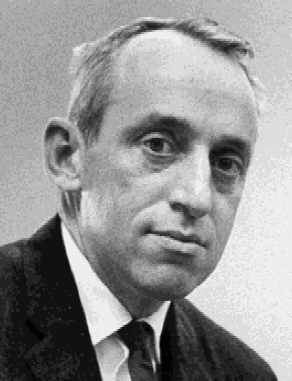
\includegraphics[width=0.3\textwidth]{./figures/aula8_fig1.png}}
        \caption{\href{https://en.wikipedia.org/wiki/James_Tobin}{James Tobin (1918 - 2002)}}
    \end{figure}    
\end{frame}

\begin{frame}
    {Teoria $q$ do investimento}
    \begin{itemize}
        \item A firma escolhe trajetória de investimento que maximiza valor presente de fluxo de lucros esperados, $V_t$:
        \begin{equation}
            \max V_t = \mathbb{E}_t\sum_{k=0}^\infty \frac{1}{(1 + r)^k}\Pi_{t+k},
            \label{aula8_eq1}
        \end{equation}
        $\Pi$ é o lucro obtido em cada período e $r$ a taxa real de juros\bigskip
        \item Para maximizar valor presente de lucros esperados, firmas devem investir até o ponto no qual benefícios marginais (BM) do investimento equalizem os custos marginais (MC)\bigskip
        \item Seja $y_t = F(N_t, K_t)$ função de produção da firma: $N$ e $K$, respectivamente, trabalho e capital\bigskip
        \item Seja $P$ o preço do produto
    \end{itemize}
\end{frame}

\begin{frame}
    {Teoria $q$ do investimento}
    \begin{itemize}
        \item Hipóteses:
        \begin{enumerate}
            \item Produto resultante do investimento e pagamento de juros, $r$, realizados ao final de cada período\medskip
            \item Estoque de capital deprecia-se a uma taxa $\delta$ em cada período e é pago no começo do período seguinte
        \end{enumerate}
        \item Benefícios marginais (MB) serão dados por:
        \begin{align}
            MB &= PF_K\left(\frac{1}{1 + r} + \frac{1-\delta}{(1 + r)^2} + \frac{(1-\delta)^2}{(1 + r)^3} + \dots\right) \nonumber \\
            &= PF_K \left(\frac{1}{1 + r}\right)\left(1 + \frac{1-\delta}{1 + r} + \frac{(1-\delta)^2}{(1 + r)^2} + \dots\right)\label{aula8_eq2}
        \end{align}
        \item Portanto:
        \begin{equation}
            MB = \frac{PF_K}{r + \delta}\label{aula8_eq3}
        \end{equation}
    \end{itemize}
\end{frame}

\begin{frame}
    {Teoria $q$ do investimento}
    \begin{itemize}
        \item Neste exemplo simples, ao decidir investir 1 unidade de $K$, assume-se que a firma paga 1 unidade pelo investimento de forma imediata\bigskip
        \item Portanto, custo marginal do investimento é igual a 1\bigskip
        \item Temos, então, que a condição de equalização de benefícios e custos marginais é dada por:
        \begin{equation}
            \frac{PF_K}{\delta + r} = 1 = \frac{MB}{MC}\label{aula8_eq4}
        \end{equation}
        \item A CPO para estoque ótimo de $K$ diz que firma deve investir até o ponto em que esta condição seja satisfeita
    \end{itemize}
\end{frame}

\begin{frame}
    {Teoria $q$ do investimento}
    \begin{itemize}
        \item Se firma investe uma unidade hoje, $\delta$ é perdido em depreciação e o resto é convertido em lucros futuros, que valem $r$ menos por unidade no período seguinte\bigskip
        \item O $q$ marginal é definido da seguinte forma:
        \begin{equation}
            q = \frac{MB}{MC} = \frac{PF_K}{\delta + r}\label{aula8_eq5}
        \end{equation}
        \begin{enumerate}
            \item Se $q > 1$: benefício excede custo marginal, firma deveria aumentar estoque de $K$ até o ponto em que $q = 1$\medskip
            \item Se $q = 1$: estoque de $K$ está no nível ótimo\medskip
            \item Se $q < 1$: firma deveria reduzir estoque de $K$\bigskip
        \end{enumerate}
        \item Hipótese de $F_{KK}(\bullet) < 0$ necessária para que sistema convirja para nível ótimo de investimento
    \end{itemize}
\end{frame}

\begin{frame}
    {Teoria $q$ do investimento}
    \begin{itemize}
        \item Note que firmas tomam decisões de investimento (\textcolor{purple}{fluxo}) selecionando estoque ótimo de capital (\textcolor{blue}{estoque})\bigskip
        \item Pequenas variações no estoque de capital desejado, portanto, podem se traduzir em grandes variações no fluxo de investimento\bigskip
        \item Uma das razões para excesso de volatilidade do investimento
    \end{itemize}
\end{frame}

\begin{frame}
    {Teoria $q$ do investimento}
    \begin{itemize}
        \item Benefícios marginais do investimento maiores quando preço unitário do produto é maior e quando investimento é mais produtivo\bigskip
        \item Pela (\ref{aula8_eq5}), firmas devem optar por aumento do investimento quando:
        \begin{enumerate}
            \item Preço do produto aumenta, $\uparrow P$\medskip
            \item Produtividade marginal do $K$ aumenta, $\uparrow F_K$ (aumento no produto que novos equipamentos de $K$ produzirão)\medskip
            \item Redução na taxa real de juros, $\downarrow r$\medskip
            \item Redução na taxa de depreciação do $K$, $\downarrow \delta$
        \end{enumerate}
    \end{itemize}
\end{frame}

\begin{frame}
    {Teoria $q$ do investimento}
    \begin{figure}
        \centering
        \href{https://core-econ.org/the-economy/book/text/14.html\#144-investment-spending}{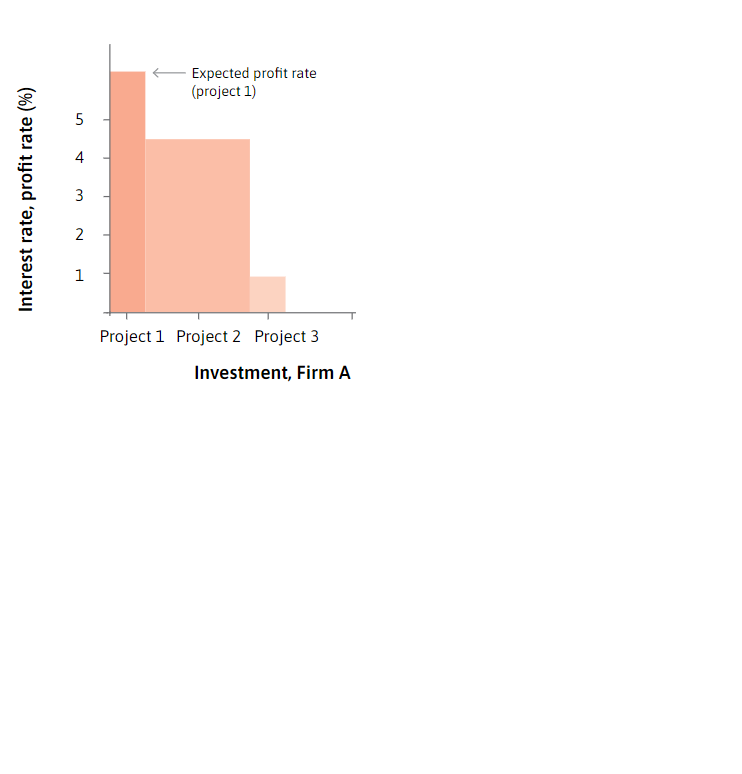
\includegraphics[width=0.4\textwidth]{./figures/aula8_fig2.PNG}}
        \caption{Investimento, taxa de lucro esperada e taxa de juros em uma economia com 2 firmas. Fonte: \href{https://core-econ.org/the-economy/book/text/14.html\#144-investment-spending}{CORE The Economy Textbook}}
    \end{figure}
\end{frame}

\begin{frame}
    {Teoria $q$ do investimento}
    \begin{figure}
        \centering
        \href{https://core-econ.org/the-economy/book/text/14.html\#144-investment-spending}{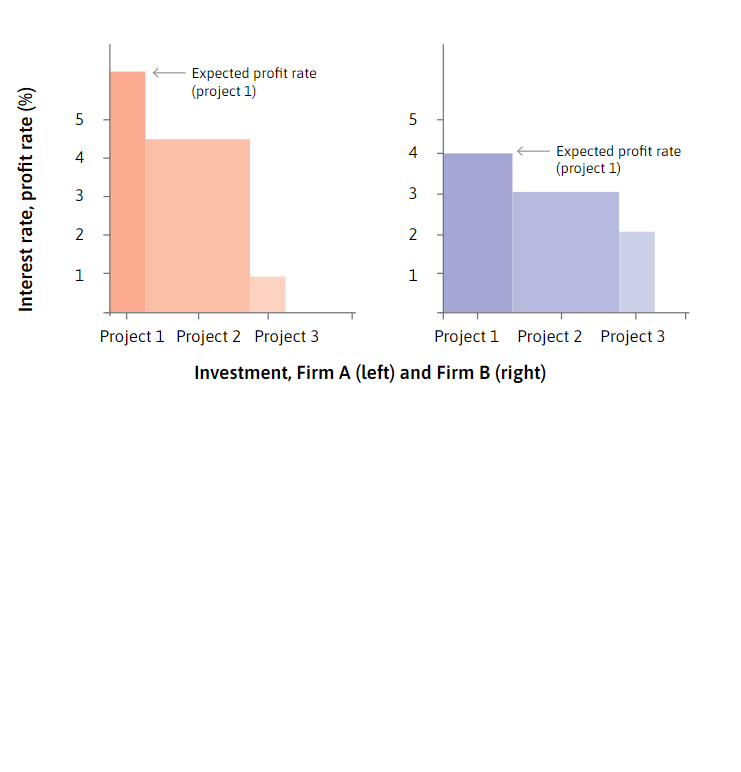
\includegraphics[width=0.4\textwidth]{./figures/aula8_fig3.PNG}}
        \caption{Investimento, taxa de lucro esperada e taxa de juros em uma economia com 2 firmas. Fonte: \href{https://core-econ.org/the-economy/book/text/14.html\#144-investment-spending}{CORE The Economy Textbook}}
    \end{figure}
\end{frame}

\begin{frame}
    {Teoria $q$ do investimento}
    \begin{figure}
        \centering
        \href{https://core-econ.org/the-economy/book/text/14.html\#144-investment-spending}{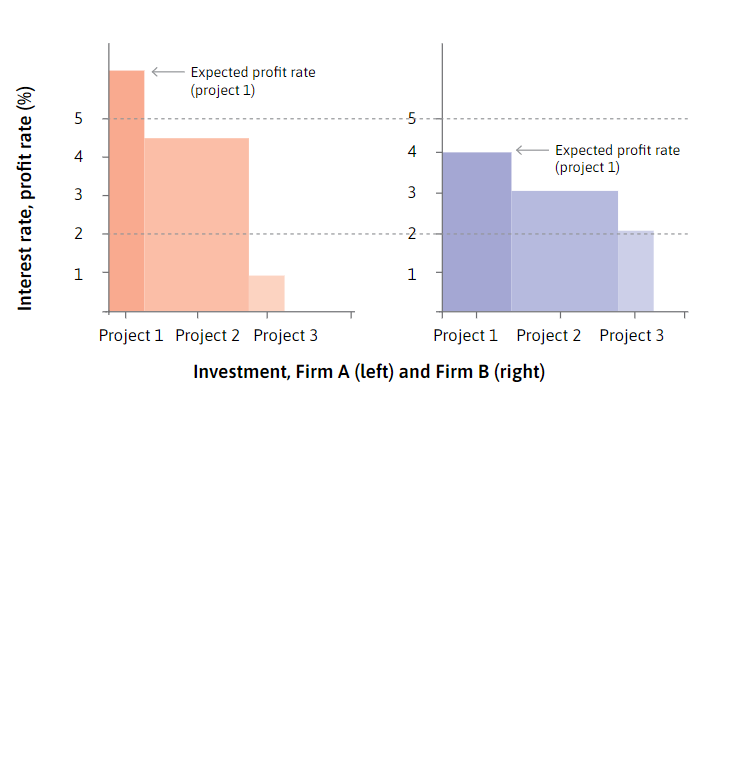
\includegraphics[width=0.4\textwidth]{./figures/aula8_fig4.PNG}}
        \caption{Investimento, taxa de lucro esperada e taxa de juros em uma economia com 2 firmas. Fonte: \href{https://core-econ.org/the-economy/book/text/14.html\#144-investment-spending}{CORE The Economy Textbook}}
    \end{figure}
\end{frame}

\begin{frame}
    {Teoria $q$ do investimento}
    \begin{figure}
        \centering
        \href{https://core-econ.org/the-economy/book/text/14.html\#144-investment-spending}{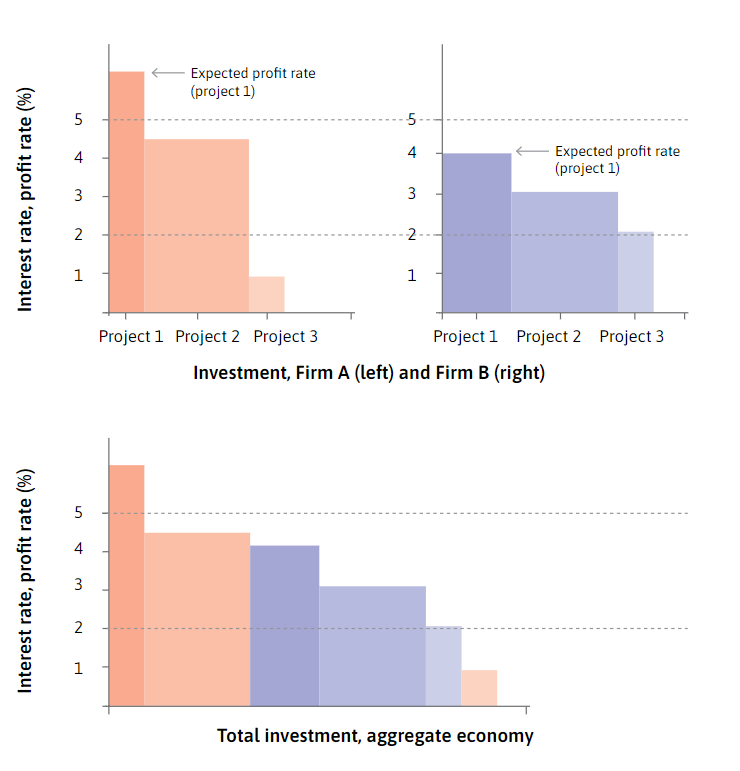
\includegraphics[width=0.4\textwidth]{./figures/aula8_fig5.PNG}}
        \caption{Investimento, taxa de lucro esperada e taxa de juros em uma economia com 2 firmas. Fonte: \href{https://core-econ.org/the-economy/book/text/14.html\#144-investment-spending}{CORE The Economy Textbook}}
    \end{figure}
\end{frame}

\begin{frame}
    {Teoria $q$ do investimento}
    \begin{figure}
        \centering
        \href{https://core-econ.org/the-economy/book/text/14.html\#144-investment-spending}{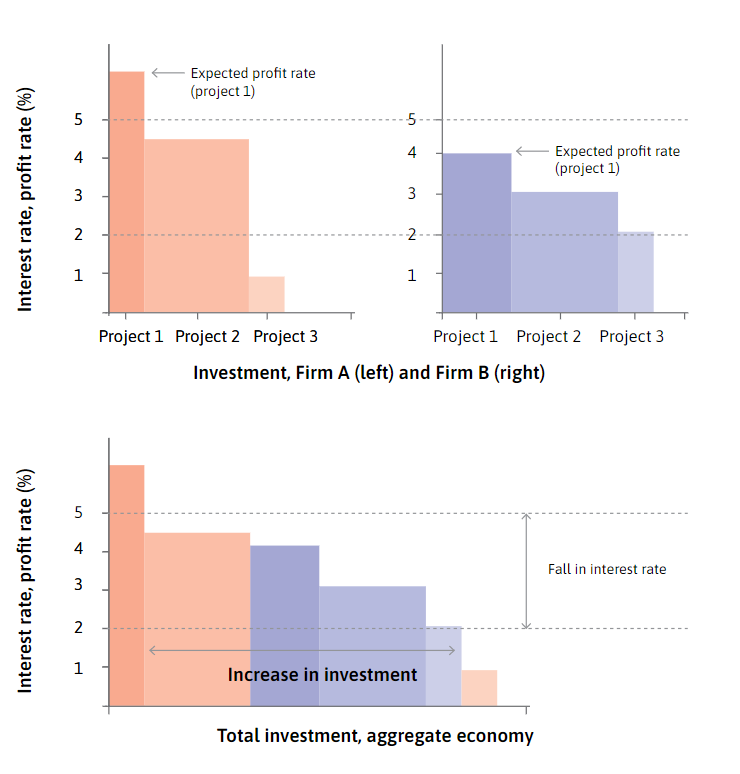
\includegraphics[width=0.4\textwidth]{./figures/aula8_fig6.PNG}}
        \caption{Investimento, taxa de lucro esperada e taxa de juros em uma economia com 2 firmas. Fonte: \href{https://core-econ.org/the-economy/book/text/14.html\#144-investment-spending}{CORE The Economy Textbook}}
    \end{figure}
\end{frame}

\begin{frame}
    {Teoria $q$ do investimento}
    \begin{figure}
        \centering
        \href{https://core-econ.org/the-economy/book/text/14.html\#144-investment-spending}{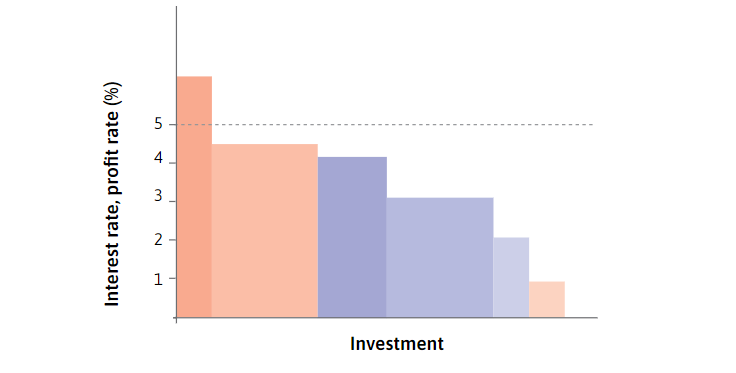
\includegraphics[width=0.6\textwidth]{./figures/aula8_fig7.PNG}}
        \caption{Investimento agregado: melhora nas condições de oferta. Fonte: \href{https://core-econ.org/the-economy/book/text/14.html\#144-investment-spending}{CORE The Economy Textbook}}
    \end{figure}
\end{frame}

\begin{frame}
    {Teoria $q$ do investimento}
    \begin{figure}
        \centering
        \href{https://core-econ.org/the-economy/book/text/14.html\#144-investment-spending}{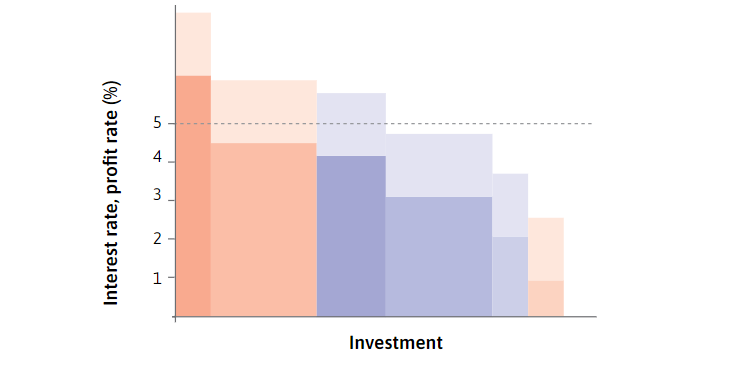
\includegraphics[width=0.6\textwidth]{./figures/aula8_fig8.PNG}}
        \caption{Investimento agregado: melhora nas condições de oferta. Fonte: \href{https://core-econ.org/the-economy/book/text/14.html\#144-investment-spending}{CORE The Economy Textbook}}
    \end{figure}
\end{frame}

\begin{frame}
    {Teoria $q$ do investimento}
    \begin{figure}
        \centering
        \href{https://core-econ.org/the-economy/book/text/14.html\#144-investment-spending}{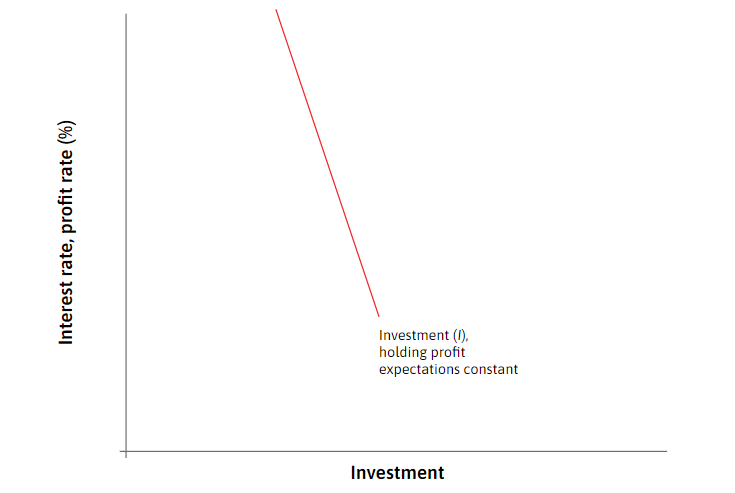
\includegraphics[width=0.6\textwidth]{./figures/aula8_fig9.PNG}}
        \caption{Função investimento agregado: efeitos de taxa real de juros e lucros esperados. Fonte: \href{https://core-econ.org/the-economy/book/text/14.html\#144-investment-spending}{CORE The Economy Textbook}}
    \end{figure}
\end{frame}

\begin{frame}
    {Teoria $q$ do investimento}
    \begin{figure}
        \centering
        \href{https://core-econ.org/the-economy/book/text/14.html\#144-investment-spending}{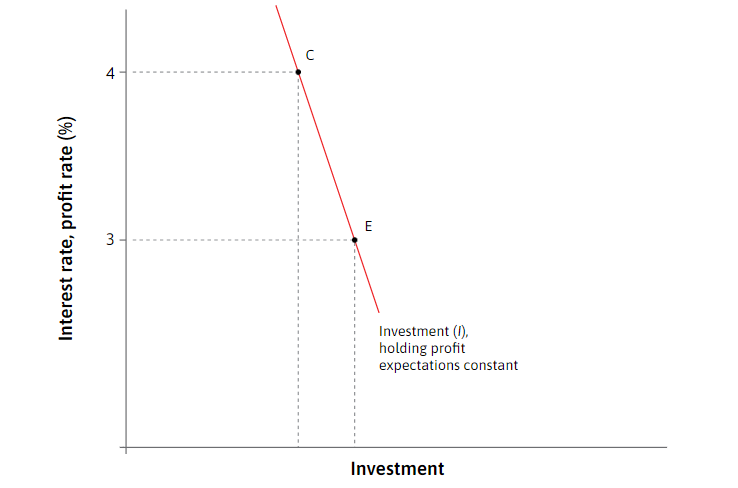
\includegraphics[width=0.6\textwidth]{./figures/aula8_fig10.PNG}}
        \caption{Função investimento agregado: efeitos de taxa real de juros e lucros esperados. Fonte: \href{https://core-econ.org/the-economy/book/text/14.html\#144-investment-spending}{CORE The Economy Textbook}}
    \end{figure}
\end{frame}

\begin{frame}
    {Teoria $q$ do investimento}
    \begin{figure}
        \centering
        \href{https://core-econ.org/the-economy/book/text/14.html\#144-investment-spending}{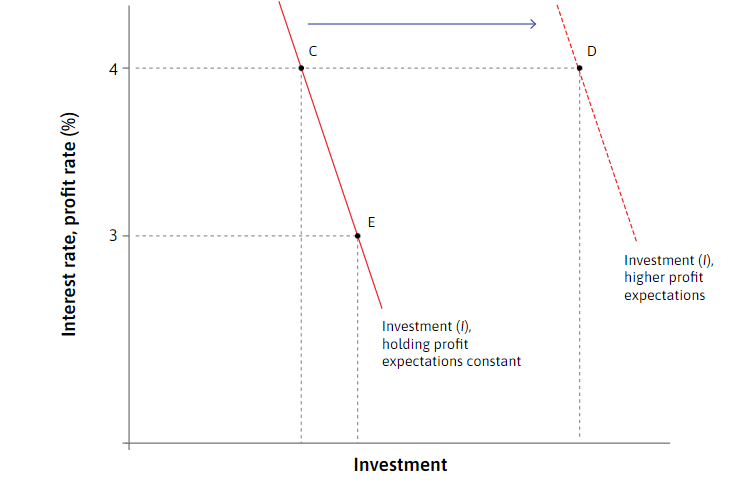
\includegraphics[width=0.6\textwidth]{./figures/aula8_fig11.PNG}}
        \caption{Função investimento agregado: efeitos de taxa real de juros e lucros esperados. Fonte: \href{https://core-econ.org/the-economy/book/text/14.html\#144-investment-spending}{CORE The Economy Textbook}}
    \end{figure}
\end{frame}

\begin{frame}
    {Teoria $q$ do investimento}
    \begin{center}
        \begin{tabular}{ |c|c|c| } 
         \hline
         Variável & Efeito sobre $q$ & Efeito sobre $I$ \\ 
         \hline
         \hline
         $r$ & $\downarrow$ & $\downarrow$ \\
         $\delta$ & $\downarrow$ & $\downarrow$ \\
         $P$ & $\uparrow$ & $\uparrow$ \\
         $F_K$ & $\uparrow$ & $\uparrow$ \\
         \hline
         %\caption{Teoria $q$ do investimento. Fonte: Carlin e Soskice (2015).}
        \end{tabular}        
        \end{center}    
\end{frame}

\begin{frame}
    {$Q$ médio}
    \begin{itemize}
        \item Teoria $q$: difícil validação empírica (função de produção e $F_K$ não observáveis)\bigskip
        \item Como operacionalizar a teoria?\bigskip
        \item \textcolor{purple}{Valor de mercado} da firma - refletido em sua avaliação no mercado de ações - é comparado ao \textcolor{purple}{cuto de reposição} do estoque de $K$\bigskip        
    \end{itemize}
\end{frame}

\begin{frame}
    {$Q$ médio}
    \begin{itemize}
        \item $Q$ médio definido da seguinte forma:
        \begin{equation}
            Q = \frac{\text{Valor de mercado}}{\text{Custo de reposição do capital}}\label{aula8_eq9}
        \end{equation}
        \item $Q$ depende do retorno esperado total do capital de uma firma dividido pelo custo total\bigskip
        \item Para empresas de capital aberto, mercado de ações fornece medida \emph{forward-looking} do valor de mercado\bigskip
        \item Se valor de mercado aumenta, relativo ao custo de reposição, refletido por um aumento no preço das ações, modelo sugere que investimento deve aumentar\bigskip
        \item Taxas de juros ou de depreciação do capital mais altos, aumentam custo de reposição
    \end{itemize}
\end{frame}

\begin{frame}
    {$Q$ médio}
    \begin{itemize}
        \item Ideia subjacente é que o valor de mercado incorpora várias informações:\bigskip
        \begin{enumerate}
            \item Quão bem espera-se que firma implemente investimento\medskip
            \item Caso novos competidores entrem no mercado\medskip
            \item Inovações tecnológicas que impactem valor da firma\medskip
            \item Estado da macro\medskip
            \item Condições de mercado de trabalho\medskip
            \item Trajetória futura da taxa de juros\bigskip
        \end{enumerate}
        \item Investir em uma empresa é uma "aposta" em um futuro incerto: investidores continuamente avaliam estes fatores e, sob condições de incerteza, o preço das ações (e valor de mercado da firma) refletirão toda informação disponível
    \end{itemize}
\end{frame}

\begin{frame}{$Q$ médio}
    \begin{tabular}{cl}
        \begin{tabular}{c}
            \href{https://ifs.org.uk/sites/default/files/output_url_files/wp0122.pdf}{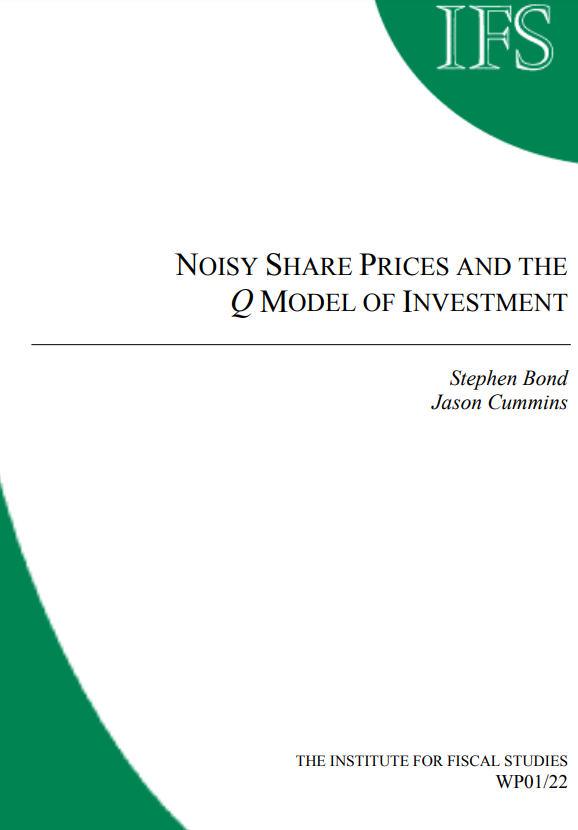
\includegraphics[width=3.5cm]{./figures/aula8_fig12.PNG}}            
        \end{tabular}
         & \begin{tabular}{l}
               \parbox{0.6\linewidth}{%  change the parbox width as appropiate
                   \begin{itemize}
                    \item Mercado de ações muito volátil\bigskip
                    \item Períodos de incerteza: preço de ações pode não refletir valor fundamental\bigskip
                    \item Grandes variações no preço de ações impactam fortemente capitalização de mercado (\emph{proxy} usada no $Q$ médio)\bigskip
                    \item Volatilidade, bolhas e comportamentos de manada no mercado de ações pode fazer com que este não seja um bom indicador de prospecções futuras\bigskip
                    \item \href{https://ifs.org.uk/sites/default/files/output_url_files/wp0122.pdf}{Bond e Cummins (2001):} microdados EUA (+ 1000 firmas de 1982-1999) - modelo $Q$ estimado com sucesso quando previsões de lucros de um analista substituem preços de ações no numerado de $Q$ 
                    \end{itemize}
               }
           \end{tabular} \\
    \end{tabular}
\end{frame}

\section{Evidências empíricas}
\begin{frame}
    {Evidências empíricas}
    \begin{itemize}
        \item $Q$ ajuda a explicar investimento, mas não é único determinante\bigskip
        \item Assim como na teoria do consumo, restrições de crédito são importantes para explicar gastos com investimento\bigskip
        \item Hipótese testável da teoria $q$: fluxo monetário corrente não deve impactar investimento\bigskip
        \item Por quê? Firmas \emph{forward looking} devem levar em consideração qualquer restrição de crédito que possuem - já deve estar incorporado na valoração de mercado $Q$\bigskip
        \item No entanto, nos estudos empíricos, papel do fluxo monetário sugere que \textcolor{purple}{imperfeições no mercado de $K$} são relevantes
    \end{itemize}
\end{frame}

\begin{frame}
    {Evidências empíricas}
    \begin{itemize}
        \item Variáveis de fluxo monetário nas equações estimadas de investimento importância similar à renda corrente nas de consumo\bigskip
        \item São evidência de que firmas se deparam com restrições de crédito\bigskip
        \item Muitas firmas são capazes de tomar empréstimos ou vender o quanto desejam para financiar planos de investimento\bigskip
        \item Mas para muitas outras, investimento é limitado por fundos internos à firma\bigskip
        \item \hlight{Excesso de sensibilidade do investimento a fundos internos}\bigskip
        \item Para essas empresas: fluxo de caixa é determinante importante dos investimentos\bigskip
        \item Aqui não discutiremos restrições a empréstimos bancários para firmas
    \end{itemize}
\end{frame}

\begin{frame}{Evidências empíricas}
    \begin{tabular}{cl}
        \begin{tabular}{c}
            \href{https://www.jstor.org/stable/2728330}{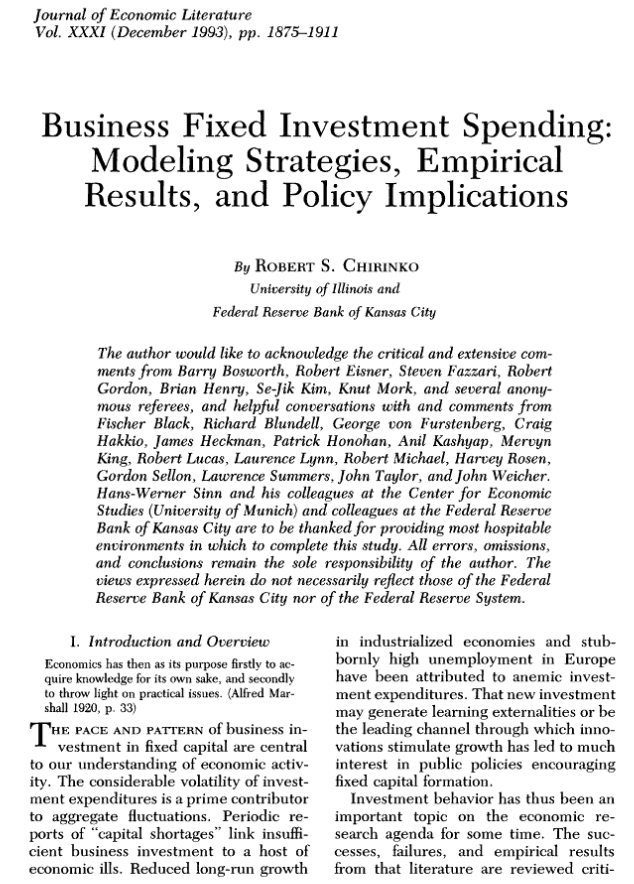
\includegraphics[width=3.5cm]{./figures/aula8_fig13.PNG}}            
        \end{tabular}
         & \begin{tabular}{l}
               \parbox{0.6\linewidth}{%  change the parbox width as appropiate
                   \begin{itemize}
                    \item Dados de empresas do UK (1975-1986) mostram que investimento é significativamente influenciado por $Q$ e restrições de crédito\medskip
                    \item Impacto de $Q$ é pequeno: aumento de 10\% no valor de mercado associado a aumento imediato na taxa de investimento de 2,5\%\medskip
                    \item Fluxos de caixa, por outro lado, muito importantes\medskip
                    \item Período amostral dividido em 2: impacto de $Q$ menor e fluxo de caixa maior na primeira subamostra (UK em profunda recessão)\medskip
                    \item Resultado compatível com importância da restrição de crédito em recessões\medskip
                    \item Ver \href{https://www.jstor.org/stable/2728330}{Chirinko (1993)}
                    \end{itemize}
               }
           \end{tabular} \\
    \end{tabular}
\end{frame}

\begin{frame}{Evidências empíricas}
    \begin{tabular}{cl}
        \begin{tabular}{c}
            \href{https://www.jstor.org/stable/2138376}{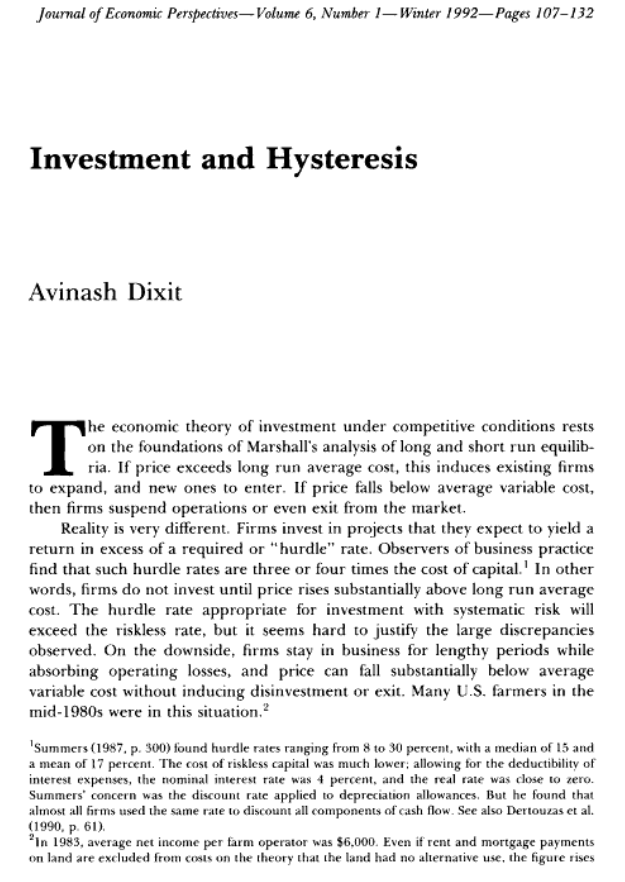
\includegraphics[width=3.5cm]{./figures/aula8_fig14.PNG}}            
        \end{tabular}
         & \begin{tabular}{l}
               \parbox{0.6\linewidth}{%  change the parbox width as appropiate
                   \begin{itemize}
                    \item Investimento também influenciado por \hlight{incerteza}\bigskip
                    \item Sob incerteza, é útil prorrogar decisões de investimento para obter novas informações\bigskip
                    \item Custos de prorrogar decisão (perda de lucros) podem ser mais que compensados por melhores informações sobre relação custo $\times$ benefício\bigskip
                    \item Portanto, uma taxa de retorno esperada consideravelmente mais alta que custo do $K$ é necessária para desencadear decisão de investimento\bigskip
                    \item \href{https://www.jstor.org/stable/2138376}{Dixit (1992)} mostra que incluir \textcolor{purple}{valor de opção de espera} pode dobrar taxa mínima (retorno necessário para desencadear investimento) para que decisão seja tomada
                    \end{itemize}
               }
           \end{tabular} \\
    \end{tabular}
\end{frame}

\begin{frame}{\emoji{books} Bibliografia}
    \begin{itemize}        
        \item BLANCHARD, O. Macroeconomia. 7.ed. São Paulo: Pearson Education do Brasil, 2017\medskip        
        \item BOND, S.; CUMMINS, J (2001). "Noisy share prices and the Q model of investment," IFS Working Papers W01/22, Institute for Fiscal Studies\medskip
        \item CHIRINKO, R. S. Business Fixed Investment Spending: Modeling Strategies, Empirical Results, and Policy Implications. Journal of Economic Literature, Vol. 31, No. 4, 1993\medskip
        \item CARLIN, W.; SOSKICE, D. Macroeconomics: Institutions, instability, and the financial system. Oxford, UK: Oxford University Press, 2015\medskip
        \item CHALLE, E. Macroeconomic fluctuations and policies. Cambridge, MA: The MIT Press, 2019\medskip
        \item DIXIT, A. "Investment and Hysteresis," Journal of Economic Perspectives, American Economic Association, vol. 6(1), 1992, pp. 107-132
    \end{itemize}
\end{frame}
\end{document}